\documentclass[pdftex,12pt,a4paper]{article}
\usepackage[utf8]{inputenc}
\usepackage[T1]{fontenc}
\usepackage{lmodern}
\usepackage{tabularx}
\usepackage{multirow}
\usepackage{graphicx}
\usepackage{hyperref}
\usepackage[ngerman]{babel}
\usepackage{booktabs,paralist}
\usepackage{scrpage2,lastpage}
\usepackage{a4wide}
\begin{document}
\newcommand{\half}{0.5\textwidth}
\newcommand{\third}{0.3\textwidth}

% Titelblatt
\begin{titlepage}
\begin{center}
\textsc{\LARGE Technische Universit\"at Dresden} \\[0.5cm]
\textsc{\LARGE Softwaretechnologie-Projekt\\[0.2cm]Gruppe 30}\\[0.7cm]
\textsc{\LARGE Geek-Shop}\\[4cm]
{\fontsize{35}{35} \bfseries Benutzerhandbuch}\\
\vspace*{\fill}
Sebastian D\"oring, Felix D\"oring, Marcus Kammerdiener,\\ Dominik Lauck, Elizaveta Ragozina\\[0.5cm]
\url{http://is63050.inf.tu-dresden.de/~swt14w30/index.php}
\end{center}
\end{titlepage}


% Inhaltsverzeichnis
\tableofcontents
\newpage

% Einführung und Ziele
\section{Einf\"uhrung und Ziele}

% Aufgabenstellung
\subsection{Aufgabenstellung} 
\textbf{„Think Nerd“ – The Shop for your nerdy needs.}\\[.25cm]
Ein echter Computer-Nerd hat ganz besondere Bedürfnisse. Wir wissen das selbst am besten. Daher haben wir uns entschlossen, einen Shop zu eröffnen, der von einfachen koffeinreichen Minzpastillen über das monatliche Linuxmagazin bis hin zur Armbanduhr mit WLAN-Empfänger alles Wichtige anbietet. „Think Nerd“ ist dabei nicht nur ein Name, sondern vielmehr unsere Geschäftsphilosophie. Schnell war klar, wir wollen ein eigens für uns entwickeltes Verwaltungssystem. Das Programm soll primär an der Kasse eingesetzt werden und den Verkaufsvorgang elektronisch abwickeln können. Bei uns gibt es nur normale Angestellte und den Ladenbesitzer.\\
Um das Geschäftsklima zu verbessern, hätten wir gern, dass jeder Angestellte mit einem zufälligem Nerd-Witz begrüßt wird. Damit sich die Witze nicht ständig wiederholen, soll der Ladenbesitzer die Möglichkeit haben, Witze entsprechend zu verwalten.\\
Einzelne Mitarbeiter sollen sich mit ihrem Namen und einem sicheren Passwort anmelden können. Unsichere Passwörter sollen bei uns gar nicht erst zugelassen werden. Ein Passwort wie „mama“ wäre also unerwünscht. Möglich wäre z. B. „MaM4.12\$“.\\
Mitarbeiter sollen vor allem Einkäufe von Kunden abwickeln. Unser Sortiment ist in Kategorien wie z. B. „Nerd-Wear“ oder „Elektronische Gagdets“ gegliedert. Die Kategorien sind ihrerseits wieder in Unterkategorien wie z. B. „Admin-Shirts“ o. „Gamer-Shirts“ unterteilt. Mitarbeiter sollen sich zunächst durch das Sortiment „klicken“ können oder über eine Suchfunktion Waren direkt finden. Angezeigte Ergebnisse sollen nach allen Kriterien (auf/absteigend nach Preis, nach Name ...) sortiert werden können, wie man es von gängigen Online-Shops her kennt. Die Angestellten sollen die Möglichkeit haben, die Waren nacheinander in einen Warenkorb einzufügen. Im nächsten Schritt sollen die Angestellten eine Übersicht über den Einkauf erhalten und die Zahlungsweise eingeben können. Es ist für Kunden möglich per elektronischem Lastschriftverfahren, per Kreditkarte oder bar zu zahlen. Nach der Bezahlung soll eine druckfertige Rechnung angezeigt werden.\\
Wir haben eine 14-tägige Geld-zurück-Garantie. Falls ein Kunde etwas reklamieren möchte, soll(en) der/die Artikel ebenfalls in einen Warenkorb gelegt werden. Im nächsten Schritt soll noch einmal die Übersicht über die Reklamation gezeigt werden. Es ist dann erforderlich, dass der Abschluss einer Reklamation vom Ladenbesitzer genehmigt werden muss. Am besten wäre es, wenn er dazu Name und Passwort eingeben müsste.\\
Der Ladenbesitzer ist für die Verwaltung der Mitarbeiter zuständig. Er kann sie entlassen, einstellen oder ihre persönlichen Daten verändern. Nur der Ladenbesitzer kann das Sortiment bearbeiten. Das hei\ss{}t er kann Kategorien und Unterkategorien erstellen, löschen und umbenennen. Ebenfalls kann nur er Artikel hinzufügen, löschen und bearbeiten.\\
Ein Überblick über den aktuellen Lagerbestand ist ebenfalls erforderlich. Der Ladenbesitzer muss den Bestand natürlich auch verändern können, um neue Lieferungen einzutragen.\\
Wenn der Bestand eines Artikels eine untere Grenze unterschreitet, möchte der Ladenbesitzer natürlich gewarnt werden.\\
Der Ladenbesitzer kann auf „Rohdaten“ aller Verkäufe zugreifen. Also wann, welcher Artikel, in welcher Menge verkauft wurde. Wir planen bei einem Freelancer ein umfangreiches Statistik-Tool für uns in Auftrag zu geben. Damit dieser gleich diese Rohdaten benutzen kann, brauchen wir eine Exportfunktion, die die Daten in eine XML Datei schreibt.

% Stakeholder
\subsection{Stakeholder}
\begin{tabularx}{\textwidth}{| *4{>{\arraybackslash}X|}} \hline
{\textbf{Rolle}} & {\textbf{Beschreibung}} & {\textbf{Ziel/Intention}} & {\textbf{Bemerkungen}}\\ \hline
Owner & Ladenbesitzer & GELD & alle Rechte\\ \hline
Employee & Mitarbeiter & Arbeiten $\rightarrow$ Geld & Sklave\\ \hline
\end{tabularx}

% Randbedingungen
\section{Randbedingungen}
% Technische Randbedingungen
\subsection{Technische Randbedingungen}
\begin{tabular}{|p{\half}|p{\half}|} \hline
\multicolumn{2}{|p{\textwidth}|}{Hardware-Vorgaben}\\ \hline
& RAM: 128 MB\\ \cline{2-2}
& Datentr\"agerkapazit\"at: 150 MB\\ \cline{2-2}
& mindestens 266MHz-Prozessor\\ \hline
\multicolumn{2}{|p{\textwidth}|}{Software-Vorgaben}\\ \hline
& Java 8\\ \cline{2-2}
& Browser mit HTML5-Unterst\"utzung\\ \hline
\multicolumn{2}{|p{\textwidth}|}{Programmiervorgaben}\\ \hline
& Java 8\\ \cline{2-2}
& Thymeleaf\\ \cline{2-2}
& Maven 3.2.5\\ \cline{2-2}
& Spring-Framework 4.1.4\\ \cline{2-2}
& SalesPoint-Framework 6.1.1\\ \hline


\end{tabular}



% Konventionen
\subsection{Konventionen}
Zur optischen Unifizierung des Codes und zur Optimierung der {\textit{Imports}} wurde die Autoformatierung von IntelliJ IDEA 14 verwendet.\\
Die Namenskonvention lautet wie folgt:\\
\begin{itemize}
\item Klassennamen beginnen mit einem Gro\ss{}buchstaben, bestehen sie aus mehreren W\"ortern, so werden sie zusammen geschrieben und jeweils der erste Buchstabe gro\ss{}
\item Methodennamen beginnen mit einem Kleinbuchstaben, bestehen sie aus mehreren W\"ortern, so werden sie zusammen und ab dem zeiten Wort die Anfangsbuchstaben gro\ss{} geschrieben.
\end{itemize}

% Kontextabgrenzung
\newpage
\section{Kontextabgrenzung}

% Fachlicher Kontext
\subsection{Fachlicher Kontext}
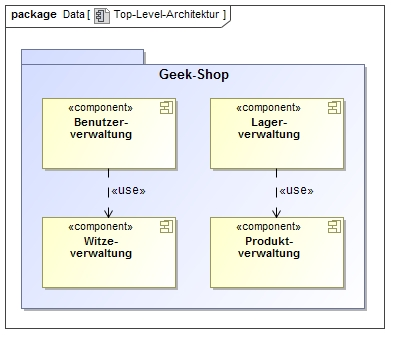
\includegraphics[width=\textwidth]{../Pflichtenheft/images/toplevelarchitektur}
Die Top-Level-Architektur besteht aus der Benutzerverwaltung, welche die Witzeverwaltung nutzt und der Lagerverwaltung, welche auf die Produktverwaltung zugreift.

% Externe Schnittstellen
\subsection{Externe Schnittstellen}
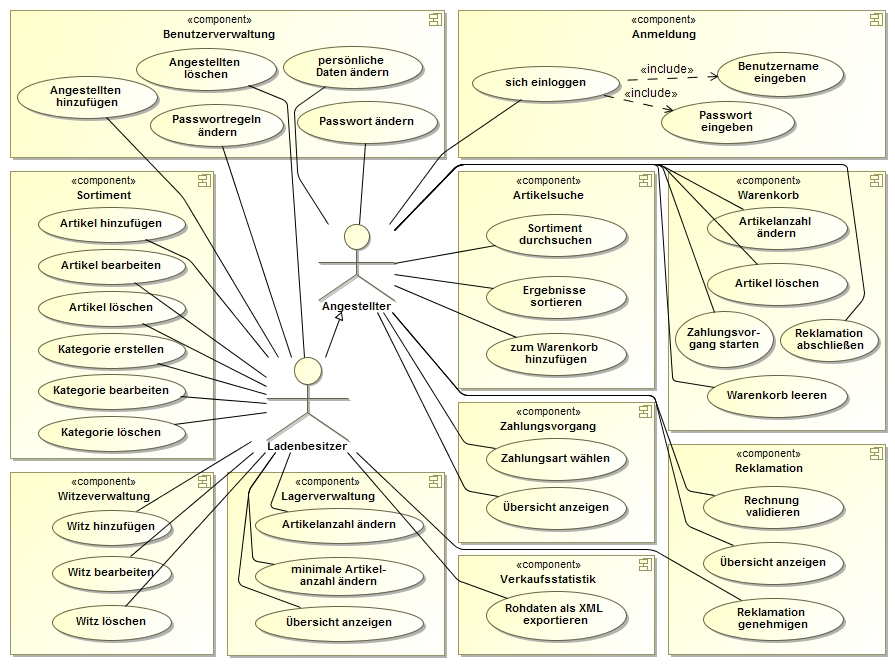
\includegraphics[width=\textwidth]{../Pflichtenheft/images/anwendungsfalldiagramm}
\vspace*{.5cm}
\begin{tabular}{|p{\third}|p{\third}|p{\third}|} \hline
{\textbf{Anwendungsfall}} & {\textbf{Beschreibung}} & {\textbf{Akteur}}\\ \hline
\multicolumn{3}{|l|}{\textbf{Benutzerverwaltung}}\\ \hline
Angestellten hinzuf\"ugen & F\"ugt einen neuen Angestellten hinzu & Ladenbesitzer\\ \hline
Angestellten l\"oschen & L\"oscht einen vorhandenen Angestellten & Ladenbesitzer\\ \hline
pers\"onliche Daten \"andern & \"Andert die pers\"onlichen Daten des Nutzers & Angestellter\\ \hline
Passwortregeln \"andern & \"Andert die Regeln der Passwortvalidierung & Ladenbesitzer\\ \hline
Passwort \"andern & \"Andert das Passwort des Nutzers & Angestellter\\ \hline
\multicolumn{3}{|l|}{\textbf{Anmeldung}}\\ \hline
sich einloggen & Loggt den Nutzer ein & Angestellter\\ \hline
\end{tabular}
\newpage
\begin{tabular}{|p{\third}|p{\third}|p{\third}|} \hline
\multicolumn{3}{|l|}{\textbf{Sortiment}}\\ \hline
Artikel hinzuf\"ugen & F\"ugt einen Artikel zum Sortiment hinzu & Ladenbesitzer\\ \hline
Artikel bearbeiten & Ver\"andert einen vorhandenen Artikel im Sortiment & Ladenbesitzer\\ \hline
Artikel l\"oschen & L\"oscht einen vorhandenen Artikel aus dem Sortiment & Ladenbesitzer\\ \hline
Kategorie erstellen & F\"ugt eine neue Kategorie hinzu & Ladenbesitzer\\ \hline
Kategorie bearbeiten & Ver\"andert eine vorhandene Kategorie & Ladenbesitzer\\ \hline
Kategorie l\"oschen & L\"oscht eine vorhandene Kategorie & Ladenbesitzer\\ \hline
\multicolumn{3}{|l|}{\textbf{Artikelsuche}}\\ \hline
Sortiment durchsuchen & Sucht Artikel aus dem Sortiment & Angestellter\\ \hline
Ergebnisse sortieren & Sortiert die gefundenen Artikel wie gew\"unscht & Angestellter\\ \hline
zum Warenkorb hinzuf\"ugen & F\"ugt Artikel zum Warenkorb hinzu & Angestellter\\ \hline
\multicolumn{3}{|l|}{\textbf{Warenkorb}}\\ \hline
Artikelanzahl \"ander & \"Andert die Anzahl des Artikels im Warenkorb & Angestellter\\ \hline
Artikel l\"oschen & Entfernt einen Artikel aus dem Warenkorb & Angestellter\\ \hline
Zahlungsvorgang starten & Beginnt den Zahlungsvorgang & Angestellter\\ \hline
Reklamation abschlie\ss{}en & Erstellt offene Reklamation & Angestellter\\ \hline
Warenkorb leeren & L\"oscht alle Artikel aus dem Warenkorb & Angestellter\\ \hline
\multicolumn{3}{|l|}{\textbf{Witzeverwaltung}}\\ \hline
Witz hinzuf\"ugen & F\"ugt einen Witz hinzu & Ladenbesitzer\\ \hline
Witz bearbeiten & Ver\"andert einen vorhandenen Witz & Ladenbesitzer\\ \hline
Witz l\"oschen & L\"oscht einen vorhandenen Witz & Ladenbesitzer\\ \hline
\end{tabular}
\newpage
\begin{tabular}{|p{\third}|p{\third}|p{\third}|} \hline
\multicolumn{3}{|l|}{\textbf{Lagerverwaltung}}\\ \hline
Artikelanzahl \"ander & \"Andert die Anzahl des Artikels im Bestand & Ladenbesitzer\\ \hline
minimale Artikelanzahl \"ander & \"Andert die  minimale Anzahl des Artikels im Bestand & Ladenbesitzer \\ \hline
\"Ubersicht anzeigen & Zeigt eine \"Ubersicht \"uber alle vorhandenen Artikel & Ladenbesitzer\\ \hline
\multicolumn{3}{|l|}{\textbf{Zahlungsvorgang}}\\ \hline
Zahlungsart ausw\"ahlen & W\"ahlt die Zahlungsart aus & Angestellter\\ \hline
\"Ubersicht anzeigen & Zeigt die Bestell\"ubersicht an & Angestellter\\ \hline
\multicolumn{3}{|l|}{\textbf{Verkaufsstatistik}}\\ \hline
Rohdaten als XML exportieren & Exportiert die Verkaufsstatistik als XML & Ladenbesitzer\\ \hline
\multicolumn{3}{|l|}{\textbf{Reklamation}}\\ \hline
Rechnung validieren & \"Uberpr\"uft, ob die Rechnung noch im Zeitrahmen liegt & Angestellter\\ \hline
\"Ubersicht anzeigen & Zeigt alle Produkte der Rechnung an & Angestellter\\ \hline
Reklamation genehmigen & Genehmigt die Reklamation und schlie\ss{}t sie ab & Ladenbesitzer\\ \hline
\end{tabular}

% Bausteinsicht
\section{Bausteinsicht}
\includegraphics[width=1\textwidth]{../../Entwurf/entwurfsklassendiagramm}

% Laufzeitsicht
\section{Laufzeitsicht}
\subsubsection*{Anmeldung}
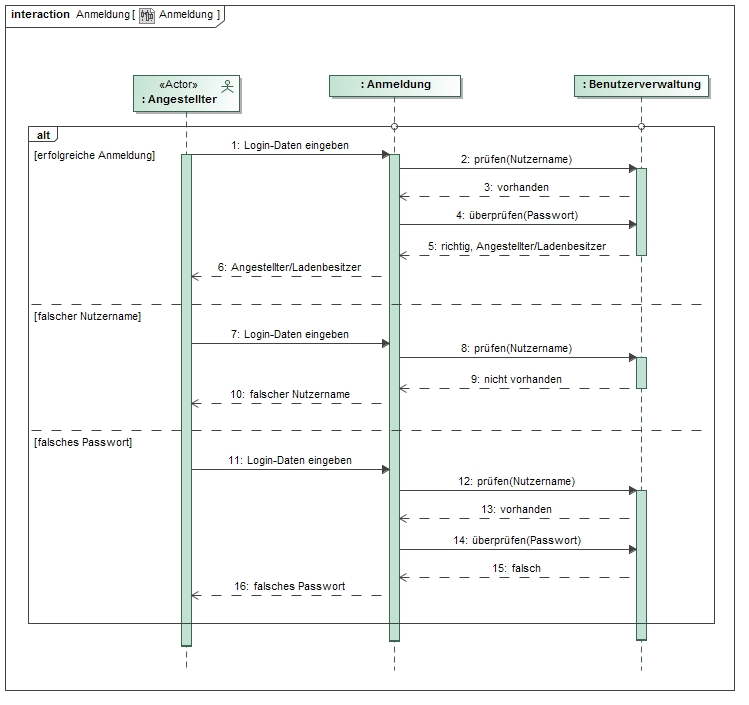
\includegraphics[width=1\textwidth]{../Pflichtenheft/images/anmeldung}
Dieses Diagramm beschreibt den Anmeldevorgang des Benutzers und wie das Programm bei einem fehlerhaften Benutzernamen oder Passwort reagiert.
\subsubsection*{Witze}
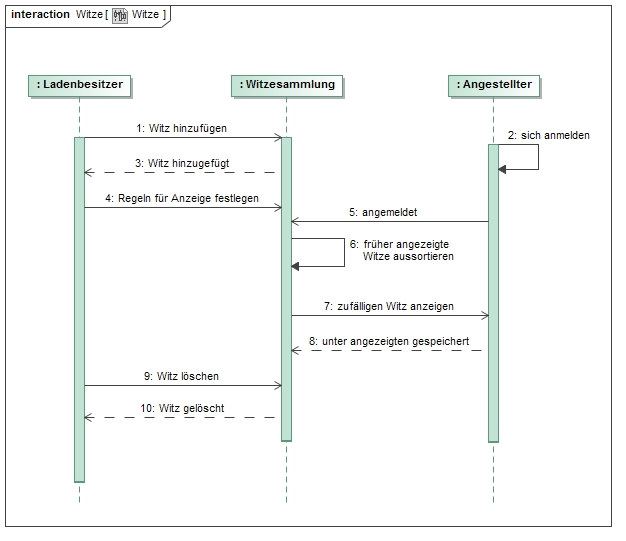
\includegraphics[width=1\textwidth]{../Pflichtenheft/images/witze}
Im oben stehenden Diagramm wird gezeigt, wie der Ladenbesitzer einen neuen Witz zur bestehenden Witzsammlung hinzufügen kann, wie ein zufälliger Witz aus der Sammlung einem Angestellten angezeigt wird und wie ein Witz aus der Sammlung gelöscht wird.
\subsubsection*{Benutzerverwaltung}
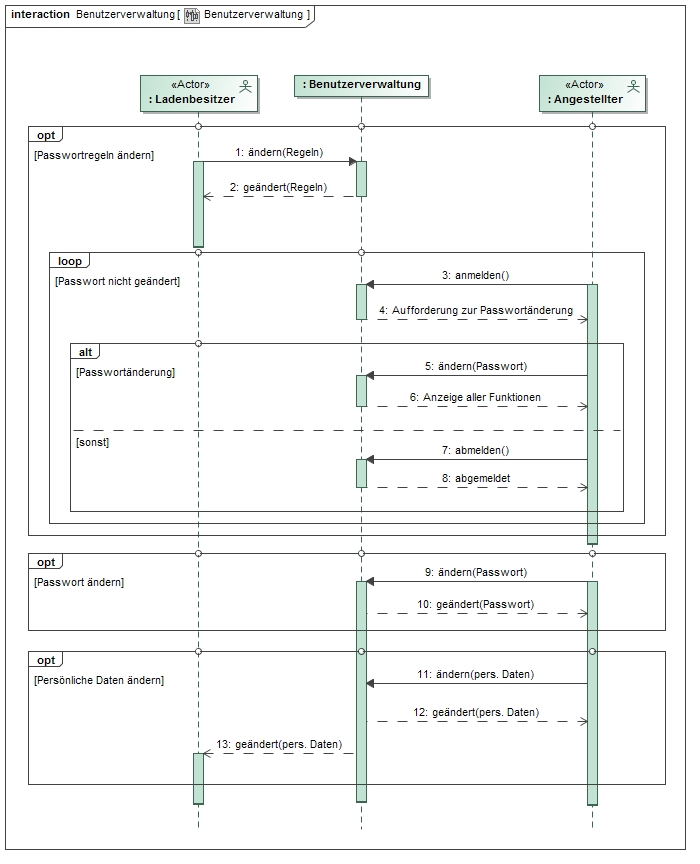
\includegraphics[width=1\textwidth]{../Pflichtenheft/images/benutzerverwaltung}
In dem Sequenzdiagramm der Benutzerverwaltung werden die M\"oglichkeit der \"Anderung der pers\"onlichen Daten und das Setzen neuer Passwortregeln sowie die dazugeh\"orige \"Anderung des Passwortes beschrieben.
\subsubsection*{Angestellten hinzuf\"ugen}
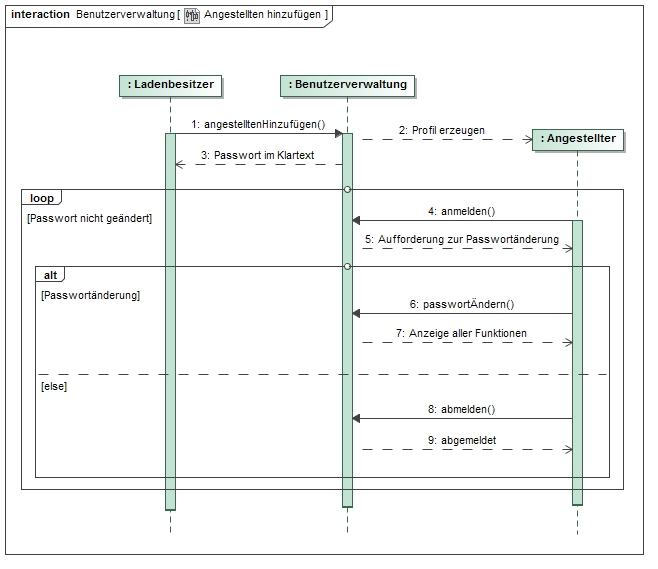
\includegraphics[width=1\textwidth]{../Pflichtenheft/images/angestelltenhinzufuegen}
Das Sequenzdiagramm zeigt den Ablauf und die Interaktion zwischen den Objekten des Systems f\"ur den Fall, dass ein neuer Mitarbeiter angelegt wird.
\subsubsection*{Angestellten l\"oschen}
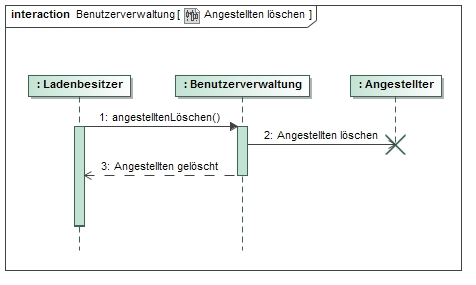
\includegraphics[width=1\textwidth]{../Pflichtenheft/images/angestelltenloeschen}
Das Sequenzdiagramm zeigt den Ablauf und die Interaktion zwischen den Objekten des Systems f\"ur den Fall, dass ein neuer Mitarbeiter gel\"oscht wird.
\subsubsection*{Kaufvorgang}
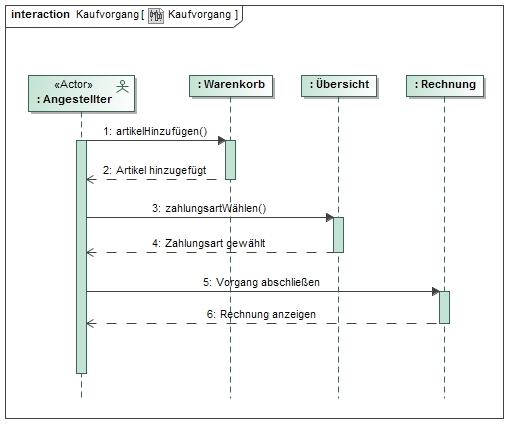
\includegraphics[width=1\textwidth]{../Pflichtenheft/images/kaufvorgang}
Dieses Diagramm zeigt, wie ein \"ublicher Kaufvorgang abl\"auft.
\subsubsection*{Reklamation}
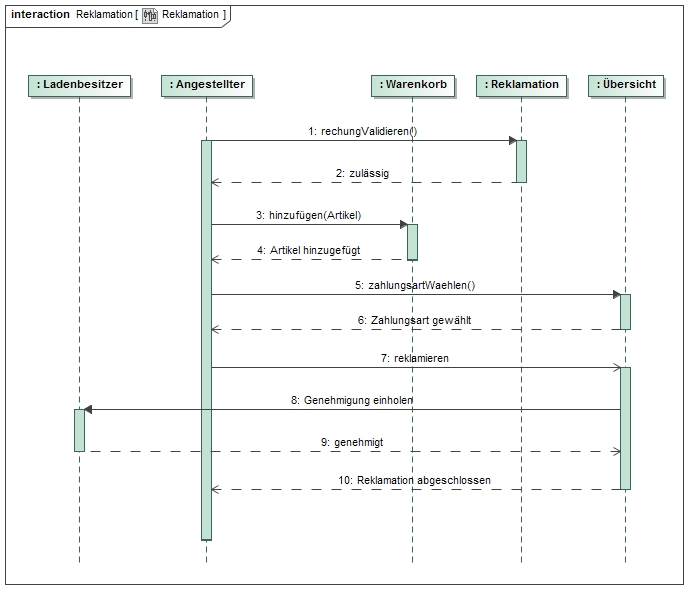
\includegraphics[width=1\textwidth]{../Pflichtenheft/images/reklamation}
Hier wird beschrieben, wie eine Reklamation abl\"auft.


% Persistenz
\subsection{Persistenz}
Die Persistenz wird mit Hilfe der Repositorys durch Spring und der in Maven integrierten Datenbank geregelt.

% Benutzungsoberfläche
\subsection{Benutzungsoberfläche}
\includegraphics[width=1\textwidth]{../Pflichtenheft/images/dialoglandkarte}

% Ergonomie
\subsection{Ergonomie}
Die Benutzeroberfl\"ache ist intuitiv gestaltet und leicht verst\"andlich.
Das Produkt wurde von der Partnergruppe mit gleichem Projekt im Crosstesting gepr\"uft.
% Transaktionsbehandlung
\subsection{Transaktionsbehandlung}
Es wurden die Transaktionen Barzahlung, Kreditkarte und Lastschrift implementiert.

% Sessionbehandlung
\subsection{Sessionbehandlung und Sicherheit}
Anhand von einer Session werden eingelogte Nutzer unterschieden. Das System basiert auf Spring Security.

% Plausibilisierung und Validierung
\subsection{Plausibilisierung und Validierung}
Alle Nutzereingaben werden \"uberpr\"uft.

% Konfigurierbarkeit
\subsection{Konfigurierbarkeit}
Der Ladenbesitzer kann jederzeit die Passwortregeln \"andern.

% Internationalisierung
\subsection{Internationalisierung}
Es wird nur die Sprache Deutsch unterst\"utzt.

% Buildmanagement
\subsection{Buildmanagement}
Der vollst\"andige Sourcecode ist auf GitHub vorhanden.



\end{document}